\subsection{BP 12:
Old  3D landslide (Laboratory)}


\subsubsection{Problem specification}

\begin{itemize}

\item PMEL-135, pp 7 \& 47-48.

%\item Problem description provided by Hermann Fritz \cite{bp8description}.

\item The original experiment is fully described on NOAA's benchmarking website which can be found at {\tt http://nctr.pmel.noaa.gov/benchmark/Laboratory/Laboratory\_Landslide/index.html}
\cite{NOAAbenchmark:3dlandslide}.

\end{itemize}

\subsubsection{What we did}

\begin{itemize}
\item We solved the nonlinear shallow water equations in Cartesian
coordinates with $g=9.81$ and no friction.

\item We used the given laboratory data and problem set up to create our
initial topography and bathymetry.  While there was data provided up to
time 20, we only conducted simulations up to time 10 as was done on 
NOAA's benchmarking website.  We specified the movement of the wedge
by using the time histories of the block motion provided for the problem.  
In order to implement this, we essentially implemented a moving bathymetry
that mimicked a wedge sliding down the linear beach.  The slope of this linear
beach was $\frac{1}{2}$.  Due to the symmetry of the problem, we simplified the
problem to half of the domain of the tank specifying an outflow or non-reflecting
boundary condition at the right boundary so reflected waves exit.  We also
specified a reflecting boundary condition at all other boundaries.
(Note that the wave tank was much longer than computational domain specified.)

\item See \Fig{bp8pcolor1} for a better picture of the problem set up.

\begin{figure}[ht]
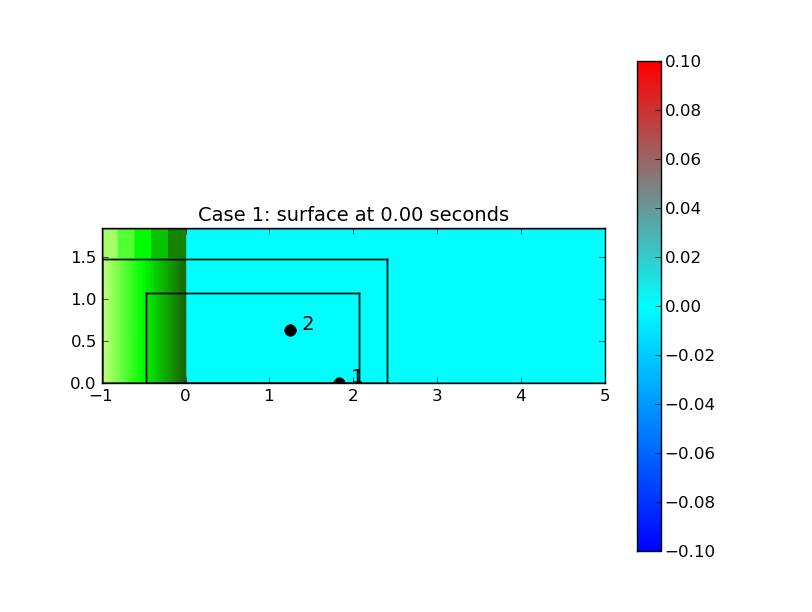
\includegraphics[width=4 in]{bp12/case1pcolor0.png}
\caption{\label{fig:bp8pcolor1}
Problem set up (top view).  Note that the black lines represent regions of 
AMR refinement with the innermost region being level 3 and the outermost
region being level 1.
  }
\end{figure}

\item We solved on $35\times 10$ grid with 3 levels of adaptive mesh refinement.
We refined in the $x$- and $y$- directions by a factor of 6 from levels 1 to 2 and
levels 2 to 3.  We refined in time by a factor of 3.  We specified level 3 refinement
on a rectangle with $x$ values of $[-0.4, 2]$ and $y$ values of $[0, 1]$.

\item We compared the simulated gauge data with the laboratory gauge data 
to determine GeoClaw's accuracy on this problem.
\end{itemize}

\subsubsection{Case 1: Simulations}

See \Fig{bp8pcolorcase1} for frames of the simulation in GeoClaw.  Note that
this only goes up to time 1.2 seconds to just get an idea of the GeoClaw
simulation.

\begin{figure}[ht]
\hfil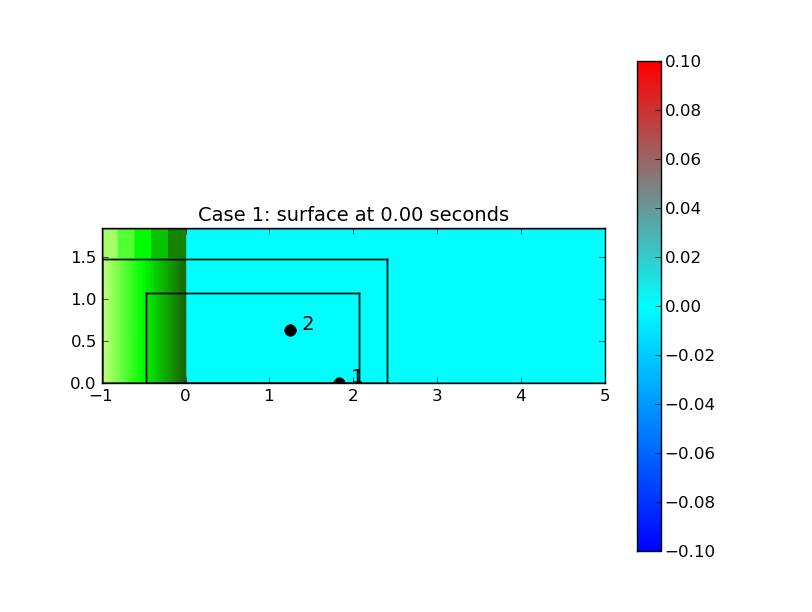
\includegraphics[width=2.8in]{bp12/case1pcolor0.png}\hfil
\hfil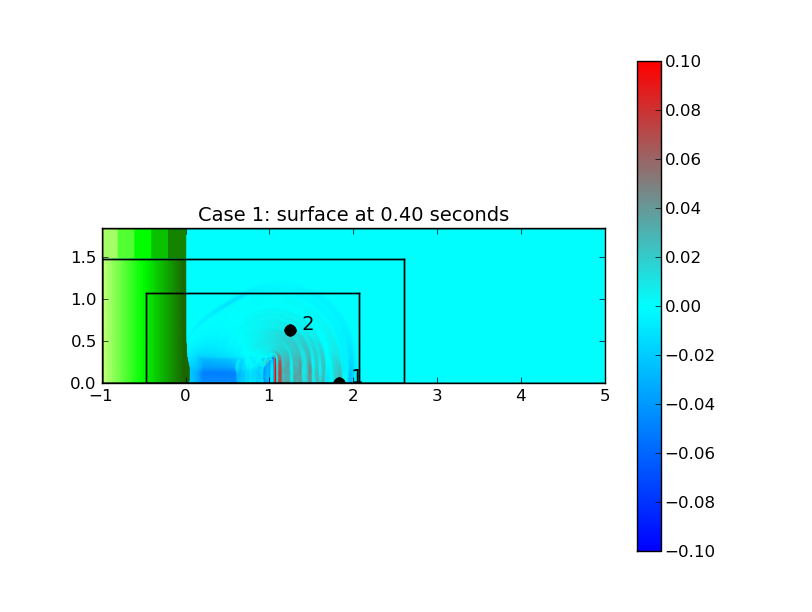
\includegraphics[width=2.8in]{bp12/case1pcolor4.png}\hfil
\vskip 5pt
\hfil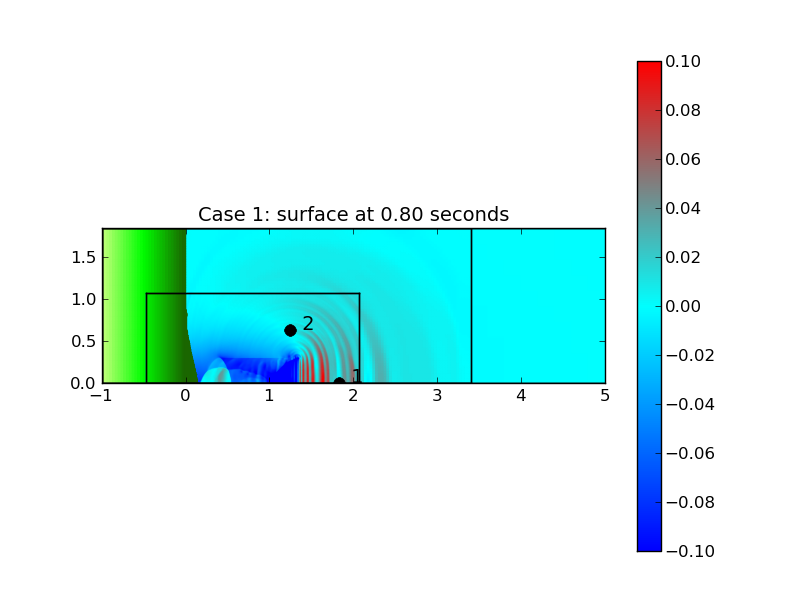
\includegraphics[width=2.8in]{bp12/case1pcolor8.png}\hfil
\hfil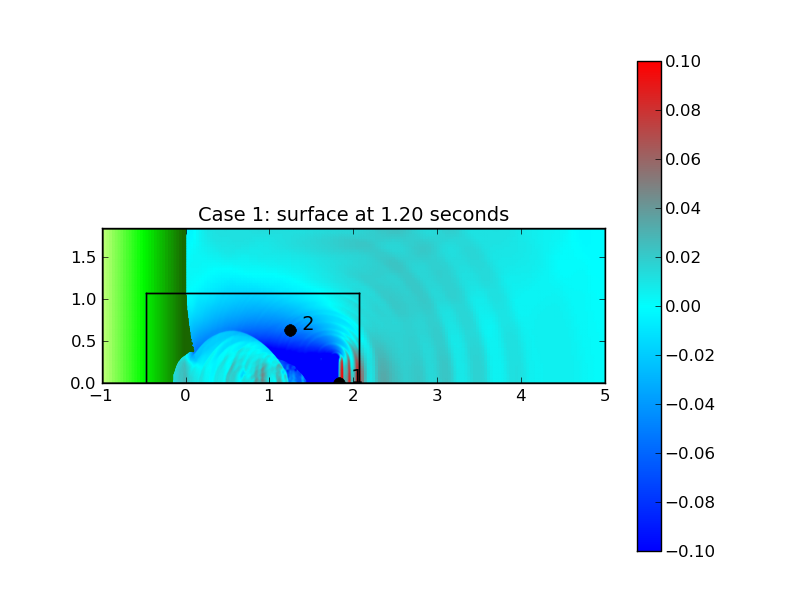
\includegraphics[width=2.8in]{bp12/case1pcolor12.png}\hfil
\caption{\label{fig:bp8pcolorcase1}
GeoClaw simulation for case 1 at times $t = 0,$ 0.4, 0.8, and 1.2.
  }
\end{figure}

\subsubsection{Case 2: Simulations}

See \Fig{bp8pcolorcase2} for frames of the simulation in GeoClaw.  Note that
this only goes up to time 1.2 seconds to just get an idea of the GeoClaw
simulation.

\begin{figure}[ht]
\hfil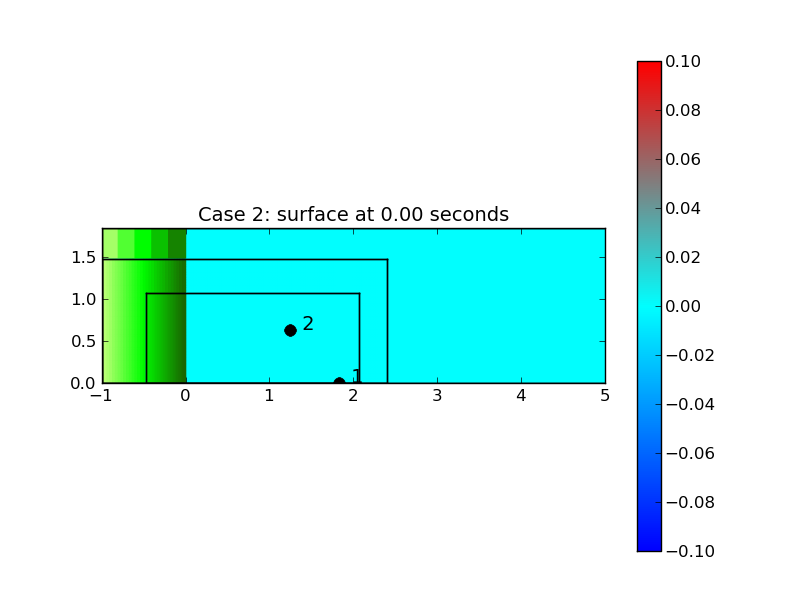
\includegraphics[width=2.8in]{bp12/case2pcolor0.png}\hfil
\hfil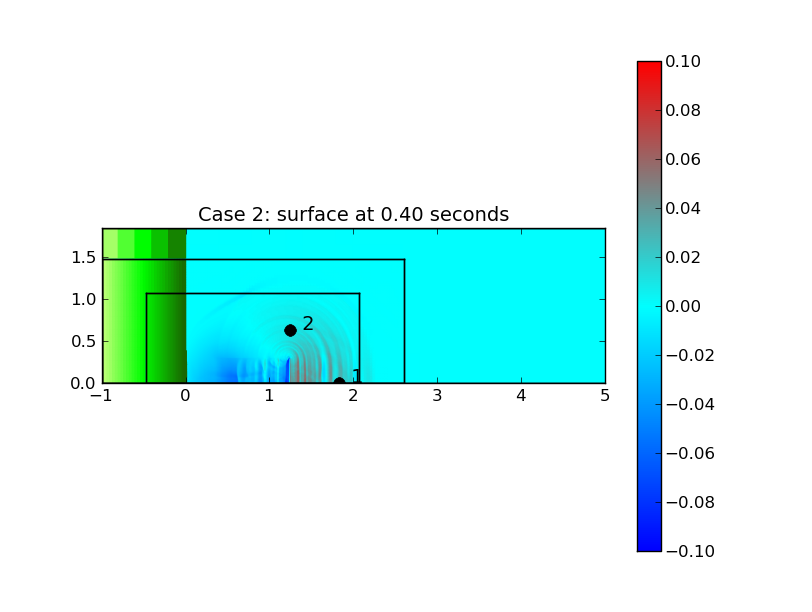
\includegraphics[width=2.8in]{bp12/case2pcolor4.png}\hfil
\vskip 5pt
\hfil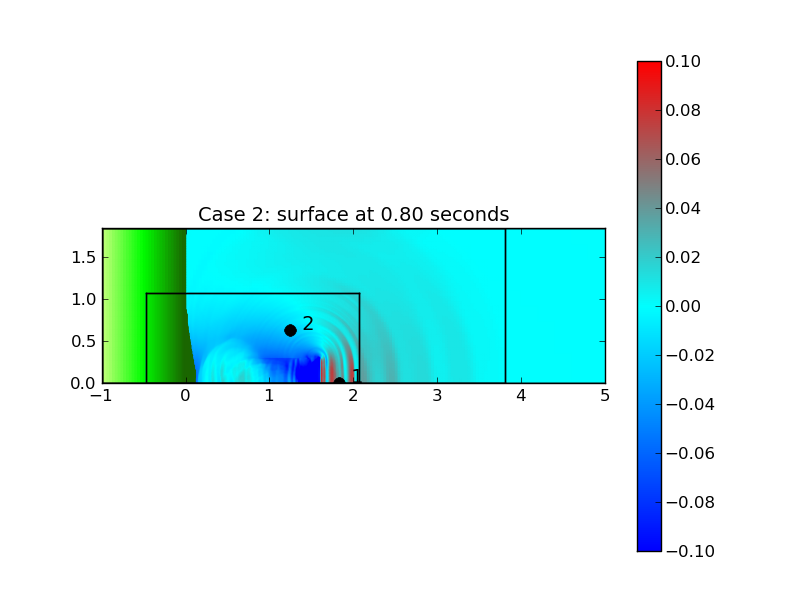
\includegraphics[width=2.8in]{bp12/case2pcolor8.png}\hfil
\hfil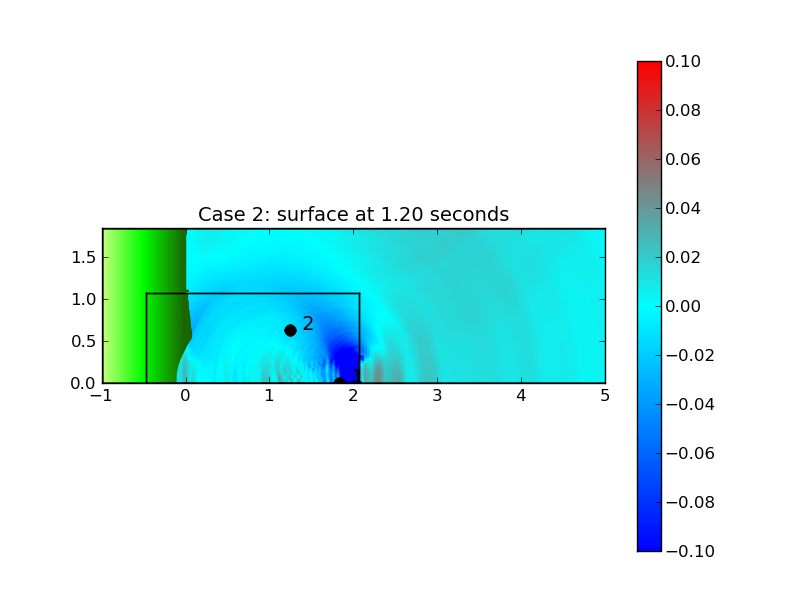
\includegraphics[width=2.8in]{bp12/case2pcolor12.png}\hfil
\caption{\label{fig:bp8pcolorcase2}
GeoClaw simulation for case 2 at times $t = 0,$ 0.4, 0.8, and 1.2.
  }
\end{figure}

\subsubsection{Case 1: Gauge comparisons}

\Fig{bp8gauges1} shows a comparison of the GeoClaw results with the
laboratory values at the two wave gauges and two runup gauges requested
for case 1.  The gauge data for gauge 1 is initially very ``noisy" but the overall
behavior seems to be captured well.  We suspect that since gauge 1 was in
the wedge's path of travel and since the wedge was specified as part of our
bathymetry, this created heavy oscillations in our wave formations.  This can
best be observed by looking at \Fig{bp8pcolorcase1} for time 0.8 seconds.
The results are in general a good match to the laboratory measurements.

\begin{figure}[ht]
\hfil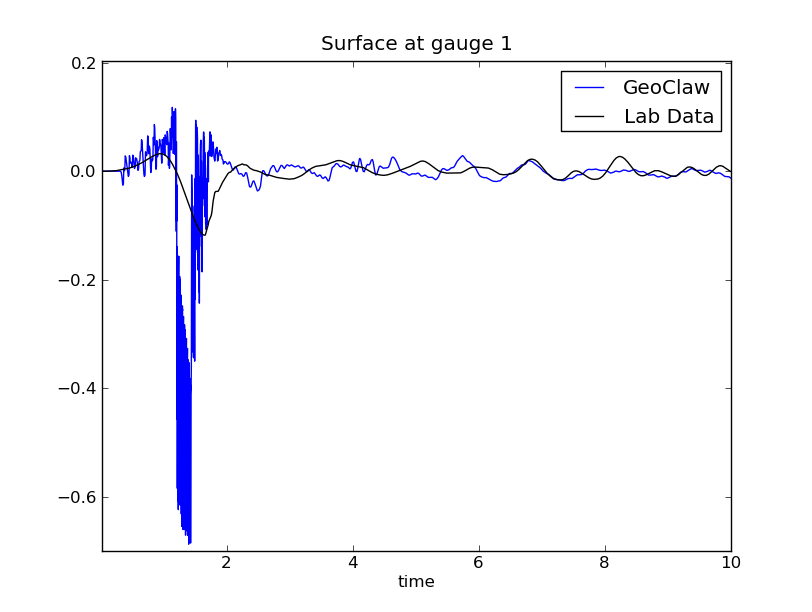
\includegraphics[width=2.8in]{bp12/case1wavegauge1.png}\hfil
\hfil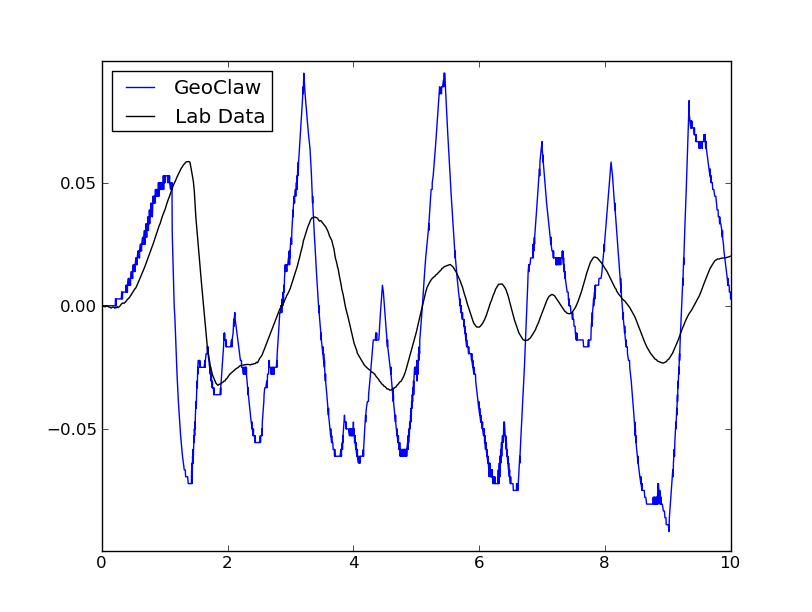
\includegraphics[width=2.8in]{bp12/case1runupgauge2.png}\hfil
\vskip 5pt
\hfil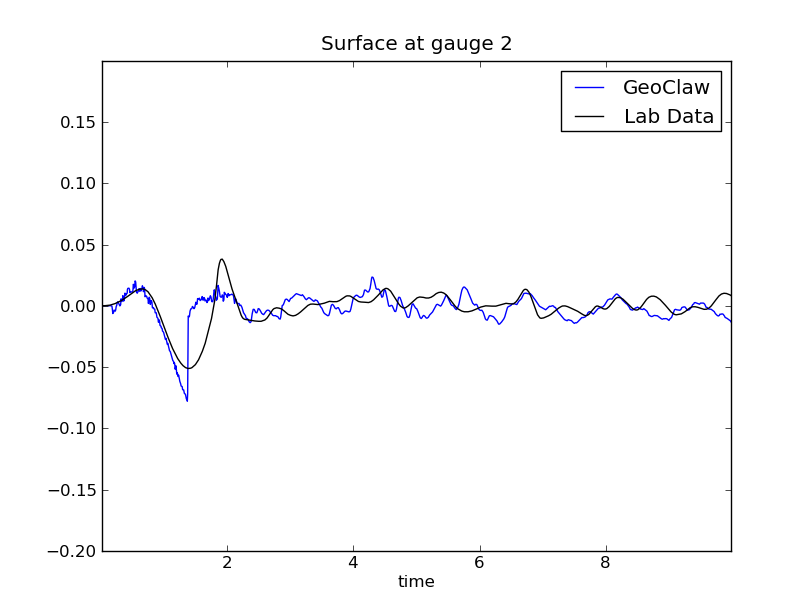
\includegraphics[width=2.8in]{bp12/case1wavegauge2.png}\hfil
\hfil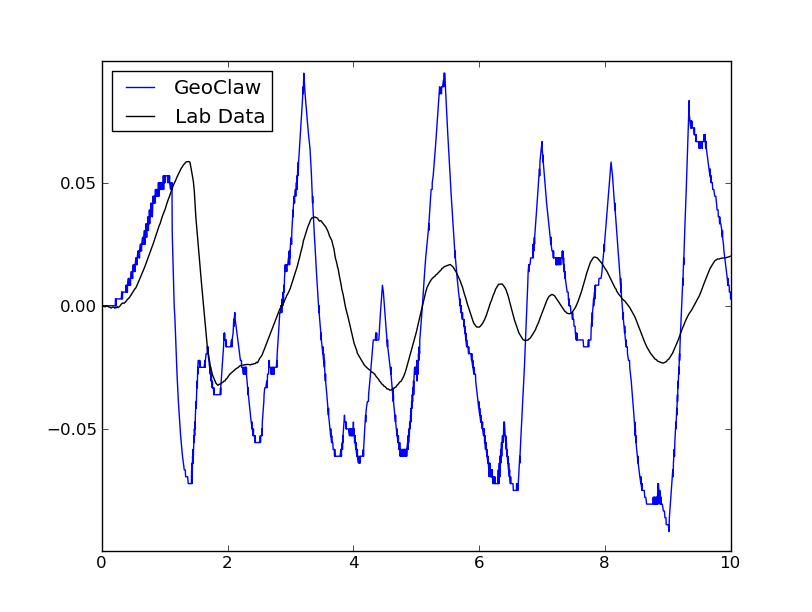
\includegraphics[width=2.8in]{bp12/case1runupgauge2.png}\hfil
\caption{\label{fig:bp8gauges1}
Left column: Time histories of the surface elevation with respect to still
water level for case 1.
Right column: Time histories of the runup measurements with respect
to still water level for case 1.
  }
\end{figure}


\subsubsection{Case 2: Gauge comparisons}

\Fig{bp8gauges2} shows a comparison of the GeoClaw results with the
laboratory values at the two wave gauges and two runup gauges requested
for case 2.  As was the case for case 1, the gauge data for gauge 1 is initially
very ``noisy" but the overall behavior seems to be captured well.  In looking at
\Fig{bp8pcolorcase2} for time 0.8 seconds, one can see why this seems to 
occur.  The results are in general a good match to the laboratory
measurements.

\begin{figure}[ht]
\hfil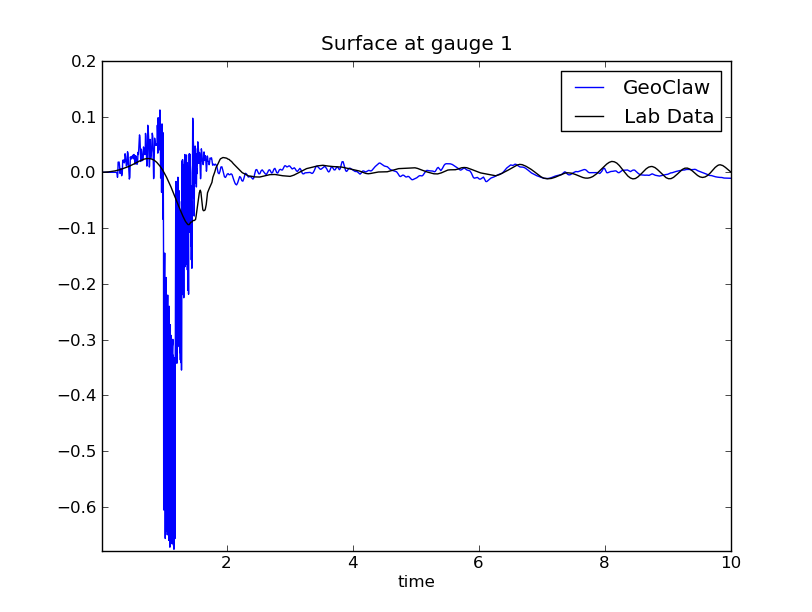
\includegraphics[width=2.8in]{bp12/case2wavegauge1.png}\hfil
\hfil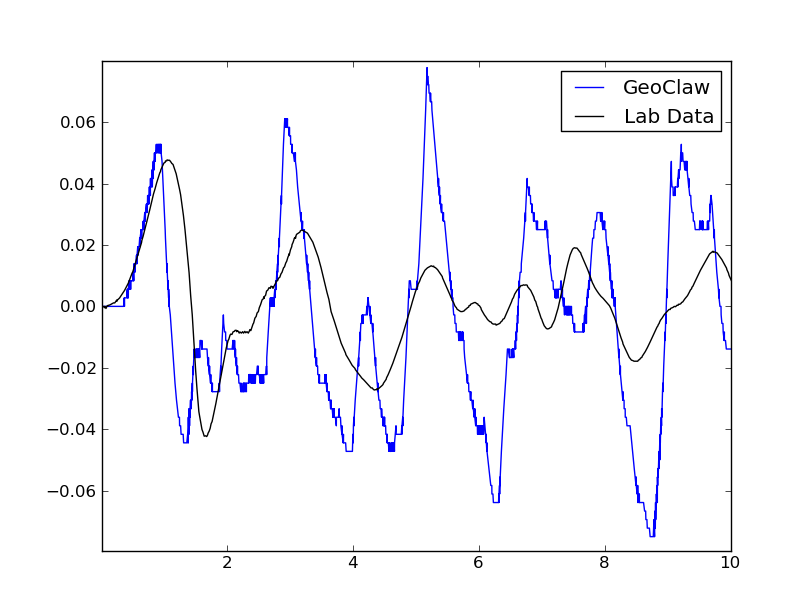
\includegraphics[width=2.8in]{bp12/case2runupgauge2.png}\hfil
\vskip 5pt
\hfil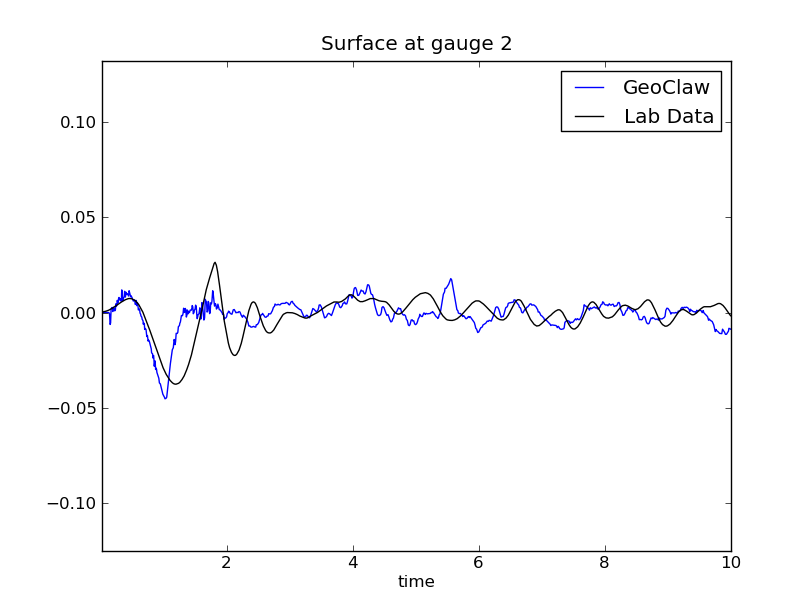
\includegraphics[width=2.8in]{bp12/case2wavegauge2.png}\hfil
\hfil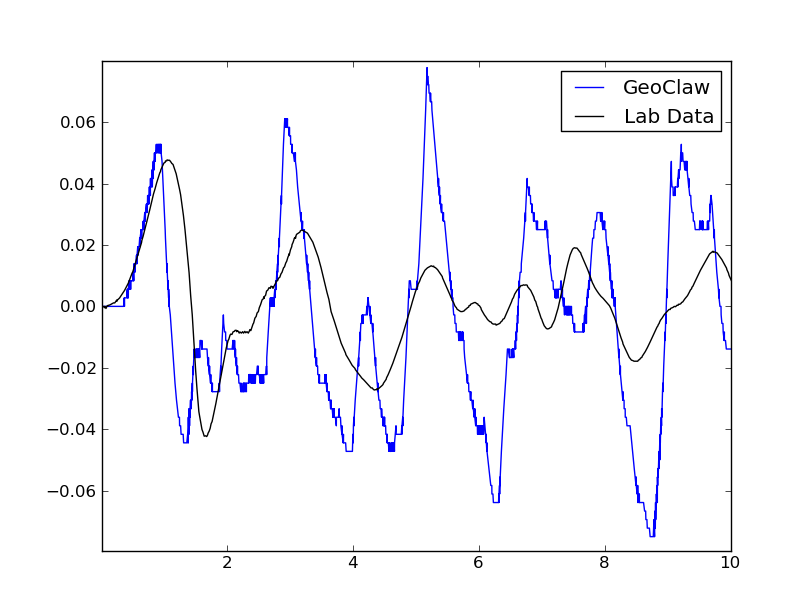
\includegraphics[width=2.8in]{bp12/case2runupgauge2.png}\hfil
\caption{\label{fig:bp8gauges2}
Left column: Time histories of the surface elevation with respect to still
water level for case 2.
Right column: Time histories of the runup measurements with respect
to still water level for case 2.
  }
\end{figure}


\subsection{Lessons learned}

\todo{Make any relevant comments or observation regarding the benchmark itself,
the available data provided, the relevance of the benchmark to tsunami
science in general and to validating your specific model in particular.
Report problems and make recommendations regarding improving the benchmark
or its data, as appropriate.}

While the data for the gauges is provided up to 20 seconds, we only use 10 seconds
of the data.

Overall, GeoClaw seems to model the surface elevations with respect to still water
level well for both cases.  However, gauge 1 seems to have issues from shortly
after the start of the simulation to about 2 seconds.  As mentioned earlier, it seems
that this phenomena is more of a result of how the bathymetry is specified than
GeoClaw's ability to model this landslide.  To smooth the data, one could try 
interpolating the data so that the moving bathymetry is smooth instead of
piecewise.  This should greatly reduce the heavy oscillations.  Another approach
would be to add a slope to the leading face of the wedge.  This would ensure a 
more gradual drop in bathymetry as the wedge propagates across the linear
beach.

It is also not clear that the shallow water equations are a good model for this
problem.  Since the beach has a constant slope of $\frac{1}{2}$, there will be a 
certain point where the depth is large.  At some distance away from the shore, 
the depth will be greater than wave length and the shallow water equations
will no longer be valid.

This benchmark problem does not appear to be a good test for tsunami models.
It has some minor issues discussed above that when rectified can make the problem
better for tsunami models that can be more accurately replicated.

